\section{Problem 3: behavioural response to playback}\label{sec:q3}

\subsection{Overall response: the paired comparison}\label{sec:q3-overall}

Table~\ref{tab:q3-rates} reports the response rates for the four outcomes. Natural calls
produce a response in 64.8\% of trials and controls in 12.9\%. The gap is not uniform across
behaviours: it is smallest for heads-up (39.6\% versus 9.4\%) and largest for approach, where
no control trial produced a single approach (16.5\% versus 0\%).

\begin{table}[htbp]
  \centering
  \caption{Response rates by outcome and stimulus (n = 139 per group), with Wilson 95\% confidence intervals.}\label{tab:q3-rates}
  \small
  \begin{tabular}{lrrrr}
    \toprule
    Outcome & Call $n$ (\%) & 95\% CI & Control $n$ (\%) & 95\% CI \\
    \midrule
    Any response & 90 (64.8) & 56.4--72.4 & 18 (12.9) & 8.4--19.5 \\
    Heads-up & 55 (39.6) & 31.8--47.9 & 13 (9.4) & 5.6--15.4 \\
    Vocalisation & 76 (54.7) & 46.4--62.8 & 5 (3.6) & 1.6--8.2 \\
    Approach & 23 (16.5) & 11.3--23.6 & 0 (0.0) & 0.0--2.7 \\
    \bottomrule
  \end{tabular}
\end{table}

Because the design is paired, the correct test compares the discordant pairs \cite{ref5}. Table~\ref{tab:q3-pair}
gives the McNemar counts. For any response, 74 pairs favour the call and 2 favour the control,
giving an odds ratio of 37.0 with an exact 95\% confidence interval of 9.9 to 311.

\begin{table}[htbp]
  \centering
  \caption{Paired McNemar tests. $b$: call responds, control does not; $c$: the reverse.}\label{tab:q3-pair}
  \small
  \begin{tabular}{lrrrrr}
    \toprule
    Outcome & $b$ & $c$ & OR & 95\% CI & Exact $p$ \\
    \midrule
    Any response & 74 & 2 & 37.0 & 9.9--311 & $<0.001$ \\
    Heads-up & 45 & 3 & 15.0 & 4.8--75.5 & $<0.001$ \\
    Vocalisation & 73 & 2 & 36.5 & 9.7--307 & $<0.001$ \\
    Approach & 23 & 0 & $\infty$ & $\geq 5.7$ & $<0.001$ \\
    \bottomrule
  \end{tabular}
\end{table}

Two robustness checks qualify this result. First, only 49 of the 139 pairs share a distance.
Restricting to those pairs lowers the odds ratio to 13.5 ($p<0.001$), which is still large but
shows that part of the apparent effect in the full sample comes from the call trials having
been played, on average, slightly closer. We report 37.0 as the design-based estimate and 13.5
as the distance-matched one; both appear in the abstract of the analysis and neither changes
the conclusion. Second, the pooled (unpaired) odds ratio is 12.4 --- close to the matched
subset (13.5) but for the wrong reason, since it ignores the matching entirely. We use the
pooled value nowhere except as an illustration of how much the design matters
(Figure~\ref{fig:q3-rates} shows the rates that underlie these comparisons).

\begin{figure}[htbp]
  \centering
  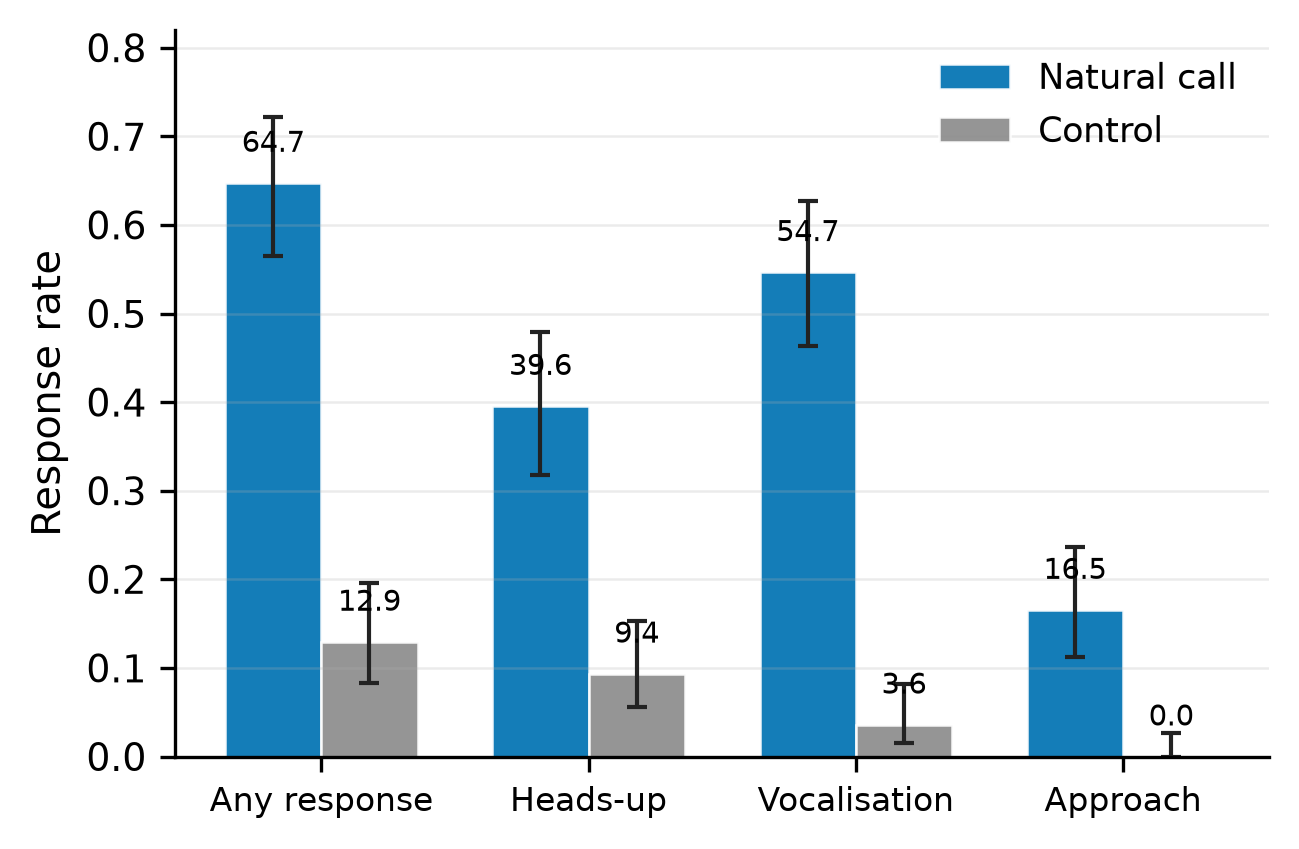
\includegraphics[width=0.40\textwidth]{figs/fig3_rates.png}
  \caption{Response rates by behaviour with Wilson 95\% confidence intervals. The approach
  outcome has no control responses at all.}\label{fig:q3-rates}
\end{figure}

\subsection{Response rates by factor level}\label{sec:q3-strata}

Before fitting a model it is worth seeing the raw structure. Table~\ref{tab:q3-strata}
cross-tabulates response against each factor within the call trials only, so that call and
control are never mixed.

\begin{table}[htbp]
  \centering
  \caption{Response rate by level of each factor, call trials only (n = 139), with Wilson 95\% confidence intervals.}\label{tab:q3-strata}
  \small
  \begin{tabular}{llrrr}
    \toprule
    Factor & Level & $n$ & Responses & Rate \% [95\% CI] \\
    \midrule
    Context & after & 36 & 19 & 52.8 [37.0, 68.0] \\
            & commuting & 65 & 35 & 53.8 [41.9, 65.4] \\
            & searching & 38 & 36 & 94.7 [82.7, 98.5] \\
    \midrule
    Call type & flat & 48 & 29 & 60.4 [46.3, 73.0] \\
              & mod & 33 & 21 & 63.6 [46.6, 77.8] \\
              & tv & 58 & 40 & 69.0 [56.2, 79.4] \\
    \midrule
    Distance & 5--30 m & 13 & 11 & 84.6 [57.8, 95.7] \\
             & 31--60 m & 49 & 31 & 63.3 [49.3, 75.3] \\
             & 61--100 m & 62 & 36 & 58.1 [45.7, 69.5] \\
             & 101--150 m & 10 & 7 & 70.0 [39.7, 89.2] \\
             & 151--200 m & 5 & 5 & 100.0 [56.6, 100.0] \\
    \midrule
    Group size & 1--3 & 39 & 35 & 89.7 [76.4, 95.9] \\
               & 4--8 & 34 & 23 & 67.6 [50.8, 80.9] \\
               & 9--15 & 32 & 21 & 65.6 [48.3, 79.6] \\
               & 16--40 & 34 & 11 & 32.4 [19.1, 49.2] \\
    \bottomrule
  \end{tabular}
\end{table}

Three features of this table drive the modelling choices. The context contrast is dramatic in
the raw data (94.7\% in searching versus about 53\% otherwise) but the searching cell contains
almost only small groups, so it cannot be read as a context effect. Distance is non-monotone:
the 101--150 m and 151--200 m bands have higher rates than the 61--100 m band, but they contain
10 and 5 trials respectively, and the 100\% cell is five trials. Group size is the only factor
with a clean monotone gradient across all four bands. This is why the multivariable model of
Section~\ref{sec:q3-factors} is necessary and why the raw table is not sufficient.

\subsection{Four factors within one framework}\label{sec:q3-factors}

The problem asks for context, call type, distance and group size to be examined in a common
model. We fit a generalised estimating equation \cite{ref4} with a logit link, an exchangeable working
correlation within experiment, and the four factors as additive terms:
\begin{equation}\label{eq:gee}
  \operatorname{logit}\,\Prob(R_{ij}=1)
  = \beta_0 + \beta_{\mathrm{CT}} + \beta_C + \beta_D \log d_{ij} + \beta_N N_{ij},
\end{equation}
where $i$ indexes the experiment and $j$ the row within it. The model uses all 278 rows and
returns population-averaged odds ratios; Table~\ref{tab:q3-gee} gives the estimates and
Figure~\ref{fig:q3-forest} displays them.

\begin{table}[htbp]
  \centering
  \caption{GEE estimates for any response (n = 278, 139 clusters). OR: odds ratio.}\label{tab:q3-gee}
  \small
  \begin{tabular}{lrrr}
    \toprule
    Term & OR & 95\% CI & $p$ \\
    \midrule
    flat vs control & 13.75 & 6.58--28.73 & $<0.001$ \\
    mod vs control & 16.28 & 6.39--41.47 & $<0.001$ \\
    tv vs control & 22.38 & 9.47--52.89 & $<0.001$ \\
    $\log$ distance (per $e$-fold) & 0.491 & 0.291--0.829 & 0.008 \\
    Group size (per bird) & 0.939 & 0.899--0.981 & 0.0045 \\
    Context: commuting vs after & 0.834 & 0.344--2.023 & 0.688 \\
    Context: searching vs after & 1.875 & 0.688--5.111 & 0.219 \\
    \bottomrule
  \end{tabular}
\end{table}

\begin{figure}[htbp]
  \centering
  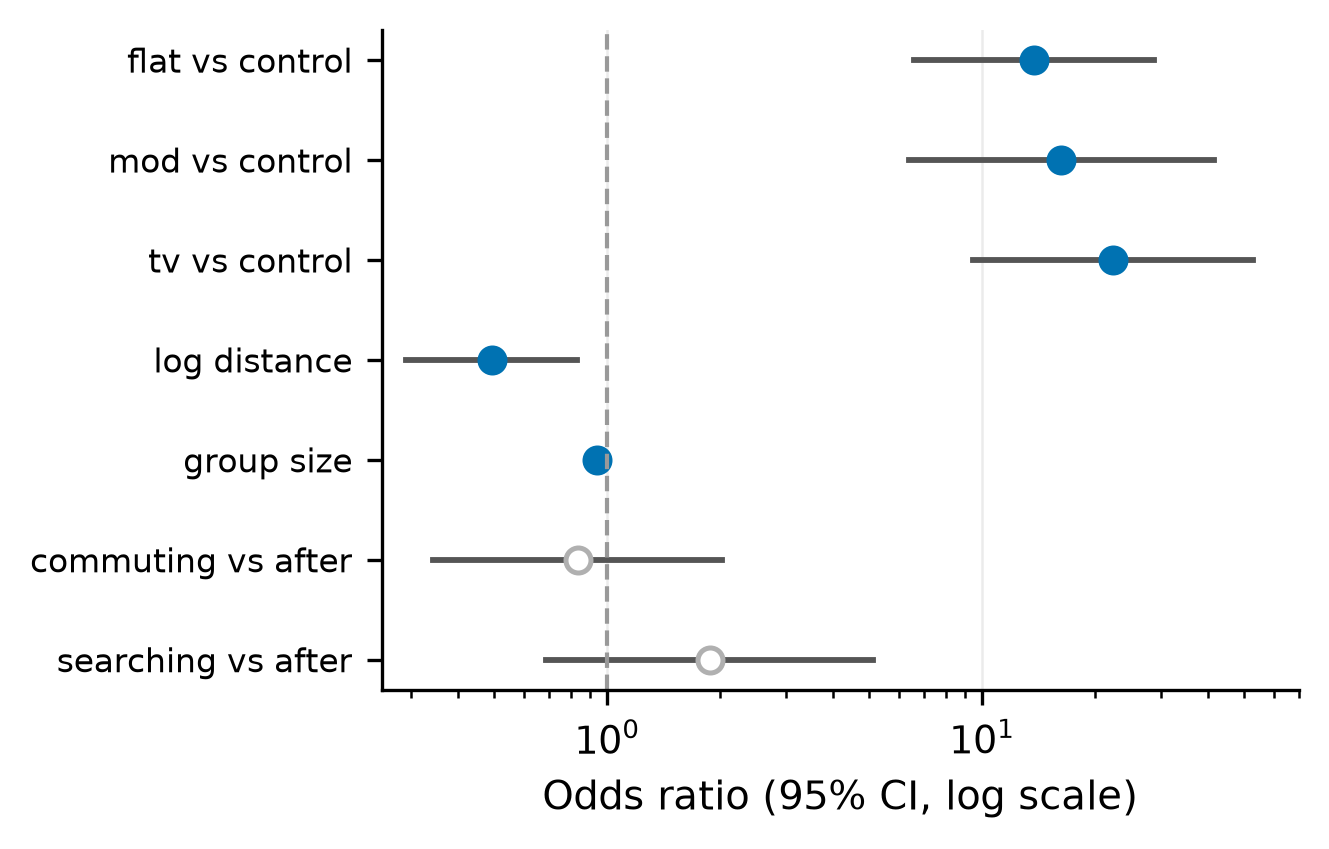
\includegraphics[width=0.40\textwidth]{figs/fig5_forest.png}
  \caption{Adjusted odds ratios from Equation~\eqref{eq:gee}. Filled markers indicate
  $p<0.05$; open markers are not significant.}\label{fig:q3-forest}
\end{figure}

Three readings matter. First, all three call types differ strongly from the control, and the
point estimates increase from flat (13.7) through modulated (16.3) to two-voice (22.4); the
confidence intervals overlap, so this ordering is suggestive rather than established. Second,
response falls with distance: each $e$-fold increase in distance multiplies the odds by 0.49,
so a bird at 140 m has roughly half the odds of responding compared with one at 50 m. Third,
and counter-intuitively, response falls with group size: each additional bird multiplies the
odds by 0.94, so a group of 20 has about half the odds of a group of 8.

Context is not significant after adjustment. This is unsurprising once the confound is seen:
the median group size is 2 in the searching context and 15 in commuting, so the raw contrast
between contexts is largely a contrast between small and large groups. We therefore report the
context coefficients but do not interpret them, and we treat group size as the substantive
variable. This is an association, not a causal effect: large groups may respond less because of
dilution of individual attention, or because an observer is less likely to detect the response
of any particular bird in a large group. The data cannot separate these mechanisms.

\subsection{The eight response combinations}\label{sec:q3-combos}

The three behaviours generate eight combinations. Table~\ref{tab:q3-combos} and
Figure~\ref{fig:q3-combos} show their distribution. The dominant pattern under playback is
vocalisation, alone or combined with heads-up; under control, 87.1\% of trials fall in the
no-response cell and the remaining cells are almost entirely heads-up only.

\begin{table}[htbp]
  \centering
  \caption{Response-combination shares. H = heads-up, V = vocalisation, A = approach.}\label{tab:q3-combos}
  \small
  \begin{tabular}{llrr}
    \toprule
    Code & Combination & Call (\%) & Control (\%) \\
    \midrule
    000 & none & 49 (35.3) & 121 (87.1) \\
    100 & H only & 10 (7.2) & 13 (9.4) \\
    010 & V only & 29 (20.9) & 5 (3.6) \\
    001 & A only & 1 (0.7) & 0 (0.0) \\
    110 & H and V & 28 (20.1) & 0 (0.0) \\
    101 & H and A & 3 (2.2) & 0 (0.0) \\
    011 & V and A & 5 (3.6) & 0 (0.0) \\
    111 & H, V and A & 14 (10.1) & 0 (0.0) \\
    \bottomrule
  \end{tabular}
\end{table}

\begin{figure}[htbp]
  \centering
  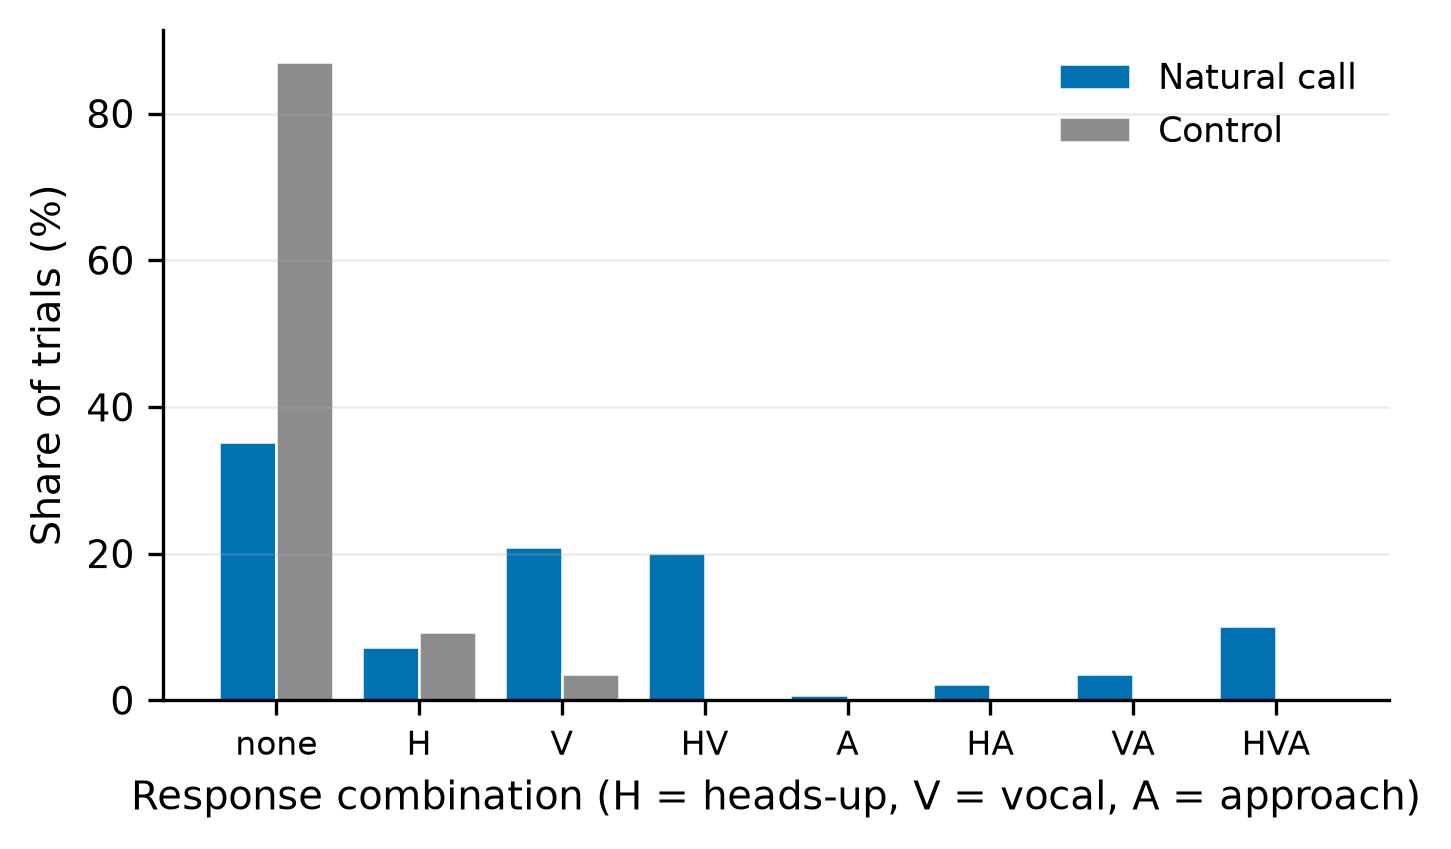
\includegraphics[width=0.42\textwidth]{figs/fig4_combos.png}
  \caption{Share of trials in each response combination.}\label{fig:q3-combos}
\end{figure}

Testing whether playback changes the distribution requires a paired test, because the two
distributions come from the same 139 experiments. A Stuart--Maxwell test \cite{ref6} on the $8\times8$
paired table gives $W=72.9$ on 7 degrees of freedom ($p<0.001$); a permutation test that swaps
call and control labels within each pair 5000 times gives $p=0.0002$. The permutation value is
the more conservative of the two and is the one we quote, because the asymptotic Stuart--Maxwell
statistic is sensitive to the many structurally empty cells.

Whether \emph{call type} shifts the probability of a \emph{specific} combination is a different
question, and here the data are thin. A contingency test of call type by combination among call
trials gives $p=0.137$, with 58\% of expected cell counts below five. We report this as a
directional observation --- two-voice calls produce more approach behaviour and less vocal-only
behaviour than flat calls --- and explicitly as a power limitation, not as evidence of
equivalence.

\subsection{Time to response}\label{sec:q3-latency}

Define the response time as the earliest of the three latencies,
$T=\min(T_H,T_V,T_A)$. A trial in which no behaviour occurs is right-censored at the observation
window $W=60$ s. Of the 108 responding trials (90 call, 18 control), nine have a latency of zero; these are immediate
reactions recorded at the resolution of the observation protocol, and we exclude them from the
latency model while reporting them separately, because a point mass at zero is not compatible
with a continuous log-normal likelihood.

The model is two-part. The first part is the response probability from
Equation~\eqref{eq:gee}. The second part is a log-normal accelerated-failure-time model fitted to
the responders with experiment-level clustering:
\begin{equation}\label{eq:aft}
  \log T_i = \beta_0 + \beta_{\mathrm{CT}} + \beta_C + \beta_D \log d_i + \beta_N N_i
  + \varepsilon_i, \qquad \varepsilon_i \sim N(0,\sigma^2).
\end{equation}
Coefficients are reported as time multipliers, $\exp(\beta)$: a value above one means a longer
time to respond.

\begin{table}[htbp]
  \centering
  \caption{Two-part log-normal AFT model for time to first response among the 99 trials that
  responded and were not immediate (90 call, 18 control, minus nine zero latencies). The reference
  category is control, so each call type is compared with the control stimulus.}\label{tab:q3-aft}
  \small
  \begin{tabular}{lrrr}
    \toprule
    Term & Time multiplier $\exp(\beta)$ & 95\% CI & $p$ \\
    \midrule
    flat vs control & 1.066 & 0.63--1.80 & 0.811 \\
    mod vs control & 0.970 & 0.58--1.63 & 0.909 \\
    tv vs control & 1.354 & 0.76--2.40 & 0.301 \\
    $\log$ distance (per $e$-fold) & 1.265 & 1.08--1.48 & 0.004 \\
    Group size (per bird) & 1.000 & 0.98--1.02 & 0.969 \\
    Context: commuting vs after & 0.810 & 0.56--1.17 & 0.259 \\
    Context: searching vs after & 0.735 & 0.49--1.10 & 0.139 \\
    \midrule
    $\sigma$ (log-scale) & \multicolumn{3}{r}{0.754} \\
    \bottomrule
  \end{tabular}
\end{table}

Only distance matters. Each $e$-fold increase in distance lengthens the expected time to
response by a factor of 1.27 (95\% CI 1.08--1.48, $p=0.004$). No call type differs from the
control stimulus, and the three call-type multipliers lie within 40\% of one another
(0.97--1.35), so call type does not detectably change latency once a bird has decided to respond;
group size does not either. This is consistent with the idea that these factors act on the
decision to respond rather than on the speed of the response.

Two summaries must be reported together, because they answer different questions. The
\emph{conditional} median latency --- the median among birds that respond --- is about 2 s for
heads-up, 3.1 s for vocalisation and 8 s for approach, with an overall first-response median of
2 s (IQR 1--4 s). The \emph{unconditional} restricted mean survival time
$\mathrm{RMST}(60)=\int_0^{60}S(t)\,dt$ \cite{ref8} keeps the non-responders in the denominator and answers
the manager's question: after a single playback, how much response time should be expected on
average? RMST is always the larger of the two numbers and cannot be smaller than the conditional
median multiplied by the response probability.

Figure~\ref{fig:q3-km} shows the Kaplan--Meier curves by call type. The curves separate mainly
in their height rather than their slope: two-voice calls leave fewer birds unanswered at every
time point, but the birds that do answer take slightly longer. This is exactly the pattern that
a single ``mean latency'' would hide, and it is why the conditional median and the RMST are
both reported.

\begin{figure}[htbp]
  \centering
  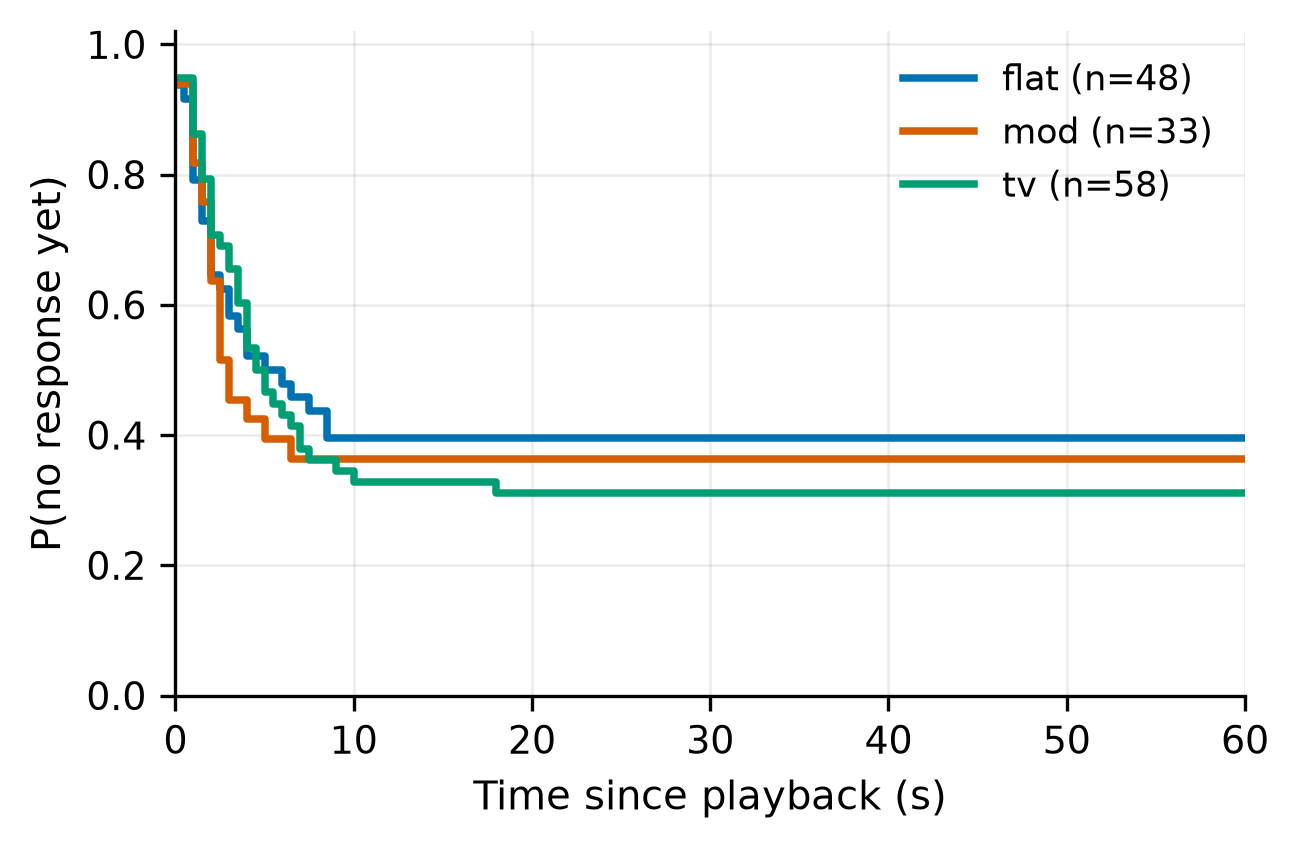
\includegraphics[width=0.40\textwidth]{figs/fig6_km.png}
  \caption{Kaplan--Meier curves of time to first response by call type, with non-responders
  censored at 60 s.}\label{fig:q3-km}
\end{figure}

\subsection{Representative numerical predictions}\label{sec:q3-table}

Table~\ref{tab:q3-pred} gives the required numerical table for a representative group of eight
penguins in the commuting context, at 50, 100 and 150 m. Every cell is a model prediction from
Equations~\eqref{eq:gee} and~\eqref{eq:aft}; none is a raw average. The response probability
falls by 11--12 percentage points from 50 to 100 m and by about 7 points from 100 to 150 m, and the ordering of call
types by response probability (two-voice $>$ modulated $>$ flat) is stable across the three
distances.

\begin{table}[htbp]
  \centering
  \caption{Predicted response probability, conditional median latency and restricted mean
  survival time. Conditions: $N=8$, commuting context.}\label{tab:q3-pred}
  \small
  \begin{tabular}{llrrr}
    \toprule
    Call type & Distance (m) & $P(\text{response})$ & Median latency (s) & $\mathrm{RMST}(60)$ (s) \\
    \midrule
    flat & 50 & 0.638 & 2.16 [1.53, 3.05] & 23.5 \\
    flat & 100 & 0.519 & 2.54 [1.75, 3.70] & 30.6 \\
    flat & 150 & 0.447 & 2.80 [1.87, 4.19] & 34.8 \\
    mod & 50 & 0.676 & 1.97 [1.35, 2.86] & 21.2 \\
    mod & 100 & 0.561 & 2.32 [1.56, 3.43] & 28.1 \\
    mod & 150 & 0.489 & 2.55 [1.67, 3.87] & 32.3 \\
    tv & 50 & 0.742 & 2.75 [2.07, 3.63] & 18.2 \\
    tv & 100 & 0.637 & 3.23 [2.41, 4.34] & 24.5 \\
    tv & 150 & 0.568 & 3.55 [2.58, 4.90] & 28.6 \\
    \bottomrule
  \end{tabular}
\end{table}

The table contains an apparent paradox worth pointing out. Two-voice calls have the highest
response probability at every distance but also the longest conditional median latency. The
reason is that the conditional median is computed among responders, while the response
probability determines how many responders there are. Once both are combined into the RMST,
two-voice calls produce the \emph{smallest} expected waiting time (18.2 s at 50 m versus 23.5 s
for flat), because more birds respond early enough to matter. Reporting only one of the three
columns would reverse the apparent conclusion.

\subsection{No response is not no perception}\label{sec:q3-perception}

The problem states that non-response must be treated as no response but must not be read as
evidence that the stimulus was not perceived. We formalise the distinction by decomposing the
response probability into a perception term and a willingness term:
\begin{align}
  \Prob(\text{response}) &= q(d)\; r(d) ,\label{eq:decomp}\\
  \Prob(\text{not perceived}) &= 1-q(d),\\
  \Prob(\text{perceived but no response}) &= q(d)\bigl(1-r(d)\bigr),
\end{align}
where $q(d)$ is the probability that the call is recognised at distance $d$ and $r(d)$ is the
probability of responding conditional on recognition.

The decomposition is useful but not identifiable from the playback data alone: for any observed
response probability one can trade a lower $q$ against a higher $r$. We therefore take $q$ from
the propagation data, as an external input, and report the result as a framework rather than as
an estimate. Two statements follow.

First, $q(d)=1$ is a hard upper bound on perception. Under that bound, at 100 m the flat call
leaves 48.1\% of trials in the ``perceived but did not respond'' category and no trial in the
``not perceived'' category. Second, the propagation-derived fidelity is \emph{not} a perception
probability: at 100 m the composite fidelity of the flat call is about 0.44, which is below the
observed response probability of 0.52. The two quantities live on different scales, and equating
them would imply a response probability exceeding the perception probability, which is
impossible. We therefore use $F(d)$ only as a monotone index of recognition difficulty and
report $q=1$ as the upper bound, with $q\in[0.5,1]$ as a sensitivity grid.

What the data do support is the qualitative statement, repeated in
Section~\ref{sec:q4}: non-response is a mixture of two mechanisms that the experiment cannot
separate, and any conservation rule that treats silence as absence of perception will
underestimate the distance at which penguins are still affected by noise.
